\documentclass{article}
\usepackage[utf8]{inputenc}
\usepackage{hyperref}
\usepackage{graphicx} % Allows including images

\title{We Rate Dogs: act report}
\author{Natalia \textsc{Bobkova}}
\date{January 2022}

\begin{document}

\maketitle

\section{Overview}

In this article we will analyze data coming from Twitter user \href{https://twitter.com/dog_rates}{@dog\_rates}, also known as \href{https://en.wikipedia.org/wiki/WeRateDogs}{WeRateDogs}. WeRateDogs is a Twitter account that rates people's dogs with a humorous comment about the dog. These ratings almost always have a denominator of 10. But what about the numerators? Almost always greater than 10. 11/10, 12/10, 13/10, etc. Why? Because of \href{http://knowyourmeme.com/memes/theyre-good-dogs-brent}{"they're good dogs Brent"} meme. WeRateDogs has over 4 million followers and has received international media coverage.

The goal of this project is to analyze WeRateDogs data and provide interesting insights and visualizations. 

\section{Data}

We have got two data sets. The first data set comes from Twitter, with all the information which can be extracted via Twitter API (such as twitter id, twitter full text, link to the post, link to the image used in the post, number of retweets and likes). Based on twitter text, some extra information was extracted, like dog rating, dog name, and dog \href{https://video.udacity-data.com/topher/2017/October/59e04ceb_dogtionary-combined/dogtionary-combined.png}{"stage"} (i.e. doggo, floofer, pupper, and puppo). 

Another data set contains the result of neural network application to predict dog's breed based on image url available in Twitter data (otherwise, dog's breed is not specified in Twitter data). We will combine Twitter data with predicted dog breeds in further exploration.

\section{Exploration}

\subsection{Prediction performances}

First, we will check up which dogs are predicted the most by the model. Golden retrievers are encountered on WeRateDogs page the most often. The top 10 predicted dog breeds includes Labradors, Pembrokes, Chihuahuas, Pugs, Chows, Samoyeds, Pomeranians, toy Puddles and Malamutes. These all are indeed very beautiful dogs, and therefore it is not surprising to find them among the most posted dogs (well, according to the model) on WeRateDogs page.

\begin{center}
    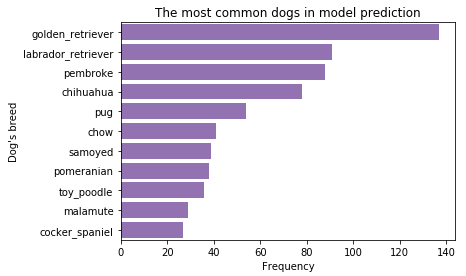
\includegraphics[scale=0.6]{preds.png}
\end{center}

\subsection{Dogs rating}

What are the most rated dogs in this page? We saw that, if the denominator is generally 10, the numerator can be higher than 10. But how much higher? In fact it can go... up to 1776! And this is not a mistake, the page rated a certain Atticus exactly like this: 1776/10. Probably, because \textit{"he's quite simply America af"} \^\^. The only flow Atticus has is that the model says it's not a dog, it's a ... bow tie.

\begin{center}
    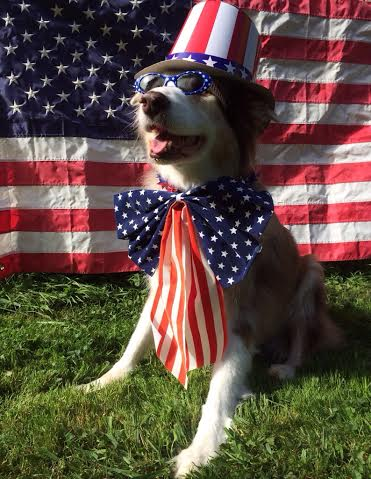
\includegraphics[scale=0.5]{rating1.jpeg}
    
\href{https://twitter.com/dog_rates/status/749981277374128128/photo/1}{Atticus} aka "bow tie"
\end{center}

The second place among the huge nominators (with a great gap though, only 420) belongs to another good dog, Snoop Dogg. The neural network model decided to support WeRateDogs in making jokes, and classified Snopp Dogg as ... microphone.

\begin{center}

\includegraphics[scale=0.4]{rating2.jpeg}

\href{https://twitter.com/dog_rates/status/670842764863651840/photo/1}{Snoop Dogg} aka "microphone"

\end{center}

\subsection{Most liked and retweeted dogs}

We had a glance over dogs (and Doggs) with the highest rating, but what about the most liked and most retweeted dogs? Here is the absolute winner in terms of both likes and retweets, the \textit{doggo realizing you can stand in a pool}. It has 71734 retweets and 146524 likes! We must admit, the model did a good job here, the doggo is classified as Labrador retriever. 

\begin{center}
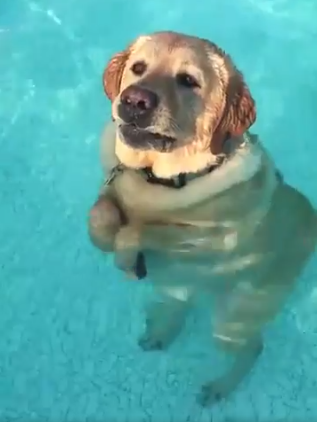
\includegraphics[scale=0.5]{golden.png}

Most liked (146.5K) and most retweeted (71.7K) \href{https://twitter.com/dog_rates/status/744234799360020481}{doggo}
\end{center}

Some cases of model errors are also  worth mentioning. 

For example, in the top 10 of the most retweeted dogs we can find the following couple, classified as swing and bubble respectively, but at least we understand why:

\vspace{20pt}
\begin{minipage}[t]{0.5\linewidth}


\includegraphics[width=0.99\linewidth]{error1.jpeg}

\centering \href{https://twitter.com/dog_rates/status/678399652199309312/video/1}{"swing"}, 29K retweets

\end{minipage}\hfill
\begin{minipage}[t]{0.5\linewidth}

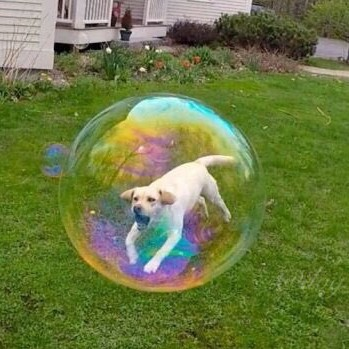
\includegraphics[width=0.99\linewidth]{error2.jpeg}

\centering \href{https://twitter.com/dog_rates/status/676219687039057920/photo/1}{"bubble"}, 28K retweets

\end{minipage}   

\vspace{20pt}

And in the top 10 of the most liked tweets we can find this cute baby Samoyed (also known as a \textit{smol polar bear}), taken for angora by the model :)

\begin{center}

\includegraphics[scale=0.5]{error3.png}

\href{https://twitter.com/dog_rates/status/859196978902773760/video/1}{"angora"}, 81.5K likes
\end{center}

\end{document}
